\graphicspath{{figures/appendix-gaspuffing/}}

\section{SUNIST 放电重复性的改善}

%\subsection{进气时序影响 SUNIST 放电重复性}

虽然 SUNIST 已经开展了一些非感应式的电流启动和维持研究\cite{TanYi:HJBYDLZTWL:ECW,TanYi2008:Thesis},现阶段欧姆放电仍然是进行物理研究时的主要运行模式。由于 SUNIST 的中心柱空间受到了极大限制,欧姆场提供的伏秒数仅能维持约 $10\,{\rm ms}$ 的等离子体,能用于进行各项研究的等离子体电流平顶段则更短。所以,在 SUNIST 中一般进行基于重复放电的多次测量,以获得感兴趣测量物理量随某个维度的变化数据\cite{WangWH2005:PPCF:Edge,HeYexi2006:PST:startup,XieHQ:2011:ISTW}。能够影响 SUNIST 放电重复性的控制手段主要包括环向、垂直、欧姆磁场的电流及投入时间和进气脉冲的宽度与时序等。在实际运行过程中,三个磁场的电流和投入时间这些电学参数可以精确控制,其重复性可以保证。经充分地放电锻炼后,真空室壁条件处于稳定,放电时的杂质行为及粒子循环等过程\cite{Belyakov2003:InpurityToPlasma:TRANSMAK}趋于稳定。但是控制压电阀门进气的电源受到了工频干扰,其电压输出存在明显的纹波,这会影响压电阀门控制的进气流速。另外,放电过程中,SUNIST 真空室内的气压处于动态变化过程中,不易得到控制。实际运行中,进气脉冲对 SUNIST 放电重复性具有明显影响\cite{TanYi2011:NF:ECR,HeYexi2006:PST:startup}。在其他装置上同样观察到了进气对放电的影响,如在 MAST\cite{Carolan:2002:MASTgaspufftoLHmode} 与 NSTX\cite{Maingi2004:PPCF:NSTXgaspufftoLHmode} 上进气位置可以影响低---高模约束的转变过程,在不同的气压下,气体击穿时对环向感应电场的要求也是不同的\cite{Chattopa1996:SINP:breakdown,Antonio2001:TCABR:breakdown}。 所以,有必要改进 SUNIST 的进气脉冲控制,进行气压分布研究,改善放电的重复性。这样不但可以获得具有重复宏观参数\pozhehao 如等离子体电流等\pozhehao 的等离子体放电,而且如气体原子激发、电离与复合等微观过程的重复性也得到了保证,有助于后续光谱实验研究中实现基于重复放电的逐炮测量。

\subsection{用于进气时序研究的相关真空硬件系统}
\label{subsec:vv-related-parts}

为了实现稳定的进气流速和研究进气脉冲后真空室内的压强变化,本文为 SUNIST 设计安装了相应的信号采集电路并重新制作了压电陶瓷阀门控制电源。相关真空硬件系统包括真空室及相关部件、气压信号采集电路和压电阀控制电源三部分。图 \ref{fig:chap04:vacuum-system} 为 SUNIST 用于进气时序研究的真空相关硬件系统示意图。

\begin{figure}
  \centering
  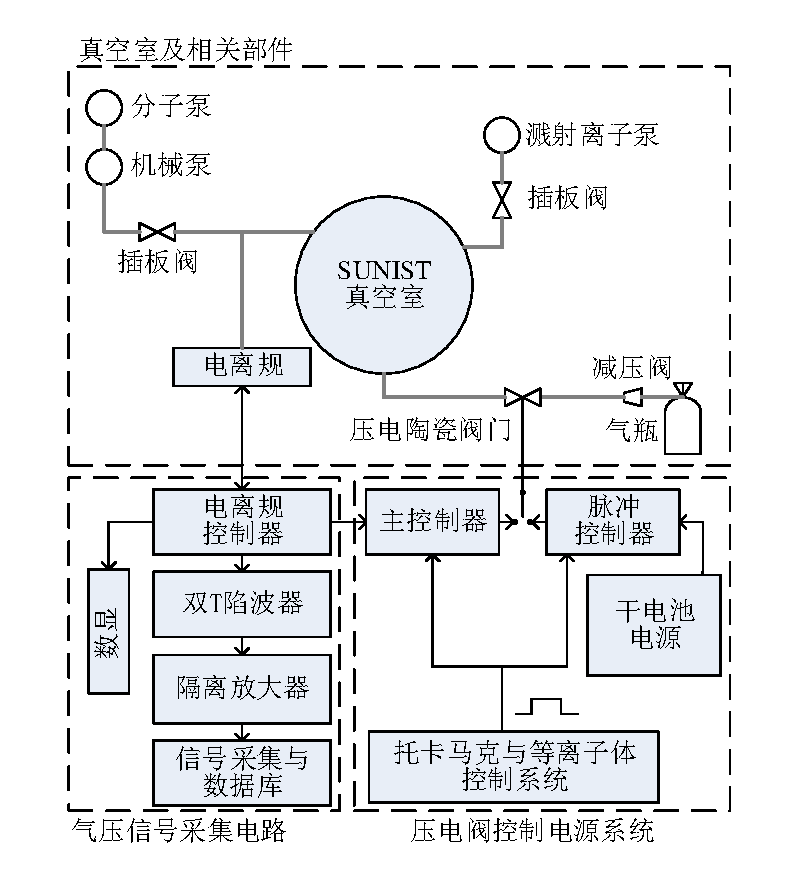
\includegraphics[width=0.8\textwidth]{vacuum-system-4.pdf}
  \caption{SUNIST 真空相关硬件系统示意图}
  \label{fig:chap04:vacuum-system}
\end{figure}

1)真空室及相关部件

图 \ref{fig:chap04:topview-vacuum-vessel} 为 SUNIST 真空室顶视图。SUNIST 使用一台分子泵做为主抽气泵。主抽气窗口上安装有直径 $d=200\,{\rm mm}$,长 $L=900\,{\rm mm}$ 的主抽气管道。在主抽气管道中间安装有一只 ZJ-27\cite{ZJ-27} 热阴极离子真空规管。在 SUNIST 真空室上部进气窗口处,通过一条直径为 $d=50\,{\rm mm}$,长为 $L=300\,{\rm mm}$ 的充气管道安装有一只 PEV-1\cite{PEV-1} 压电陶瓷阀门。其中,主抽气窗口与充气窗口沿环向呈 $120^\circ$ 角。当主抽气分子泵停止运行时,使用一台溅射离子泵维持真空本底。

\begin{figure}
  \centering
  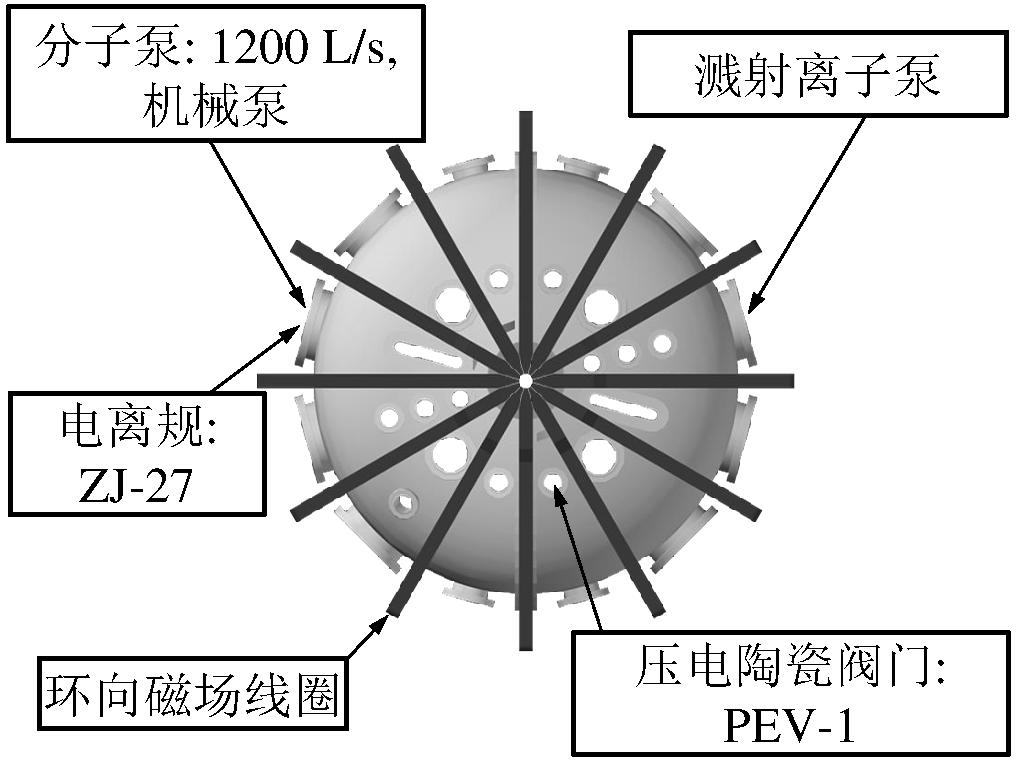
\includegraphics[width=0.6\textwidth]{topview-vacuum-vessel.pdf}
  \caption{SUNIST 真空室顶视图,修改自 \onlinecite{TanYi2013:1stA3}。}
  \label{fig:chap04:topview-vacuum-vessel}
\end{figure}


2)气压信号采集电路

电离规控制器有三个作用:a)为电离规管提供电源;b)将电离规管输出处理为气压信号,并通过数码显示管以 $1\,{\rm Hz}$ 的频率慢速显示;c)输出快速气压模拟量信号。真空室气压快速信号可以用来分析真空室内的气压流动,通过对脉冲进气后真空室内部气压分布变化情况,选择合适的进气脉冲宽度和时序以改善放电重复性。

\begin{figure}%[H]
  \centering
  \rotatebox{270}{\includegraphics[height=0.8\textwidth]{50Hz-notch-filter.pdf}}
  \caption{SUNIST 上使用的去除气压信号中工频干扰的无源双 T 陷波器电路图}
  \label{fig:chap04:50HzNotchFilter}
\end{figure}

然而,真空规控制器输出的气压信号受到强烈的 $50\,{\rm Hz}$ 电网工频干扰。要去除电源线带来的干扰,可以串入无源双 T 陷波器(passive twin-T notch filter,图 \ref{fig:chap04:50HzNotchFilter}),其传输特性计算结果如图 \ref{fig:chap04:BodeDiagram50HzNotchFilter} 所示,由于使用的电阻和电容实际值与设计有偏差,陷波器的中心截止频率为 $50.9\,{\rm Hz}$。实际测量结果显示,该陷波器可以很好的消除气压信号中的工频干扰(图 \ref{fig:chap04:50hz-trapping})。气压信号的变化频率为 $10\,{\rm Hz}$ 量级,陷波器会在此频率的信号上引起约 $70^\circ$ 的相位延迟(图 \ref{fig:chap04:BodeDiagram50HzNotchFilter}(b))。图 \ref{fig:chap04:50hz-trapping} 显示的加入陷波器后引起的 $\sim21\,{\rm ms}$ 信号延迟与陷波器的传输特性计算结果相吻合。

\begin{figure}
  \centering
  \begin{overpic}[width=0.7\textwidth]{50Hz-notch-filter-Bode-Diagram.pdf}
    \put(42,0.7){\mbox{\colorbox{white}{\quad 频率 (Hz) \quad}}}
    \put(0.7, 18.5){\rotatebox{90}{\mbox{\colorbox{white}{相位 ($^\circ$)}}}}
    \put(0.7, 49){\rotatebox{90}{\mbox{\colorbox{white}{\quad 增益\quad}}}}
  \end{overpic}
  \caption{双 T 陷波器伯德图(bode diagram)}
  \label{fig:chap04:BodeDiagram50HzNotchFilter}
\end{figure}

\begin{figure}
  \centering
  \begin{overpic}[width=0.7\textwidth]{50hz_trapping.pdf}
    \put(42,0){\mbox{\colorbox{white}{\small 时间 (${\rm ms}$)}}}
    %\put(63, 38){\mbox{\colorbox{white}{\small 平滑处理}}}
  \end{overpic}
  \caption{气压信号 $p_{\rm gas}$ 在加陷波器(w/ twin-T)与不加陷波器(w/o twin-T)情况下的测量结果,进气脉冲以灰度条表示。}
  \label{fig:chap04:50hz-trapping}
\end{figure}

放电过程中,气压信号的地电位会随着真空室浮动。在真空测量系统与数据采集系统之间加入隔离运放,不但可以将气压信号地电位与数据采集系统隔离,保护数据采集系统,而且可以用来驱动气压测量设备与数据采集系统之间的长导线。

电离规控制器输出的信号幅值与气压关系标定结果在图 \ref{fig:chap04:GasSignalCalibration} 中画出,拟合结果为:
\begin{equation}
  p_{\rm gas}(10^{-3}\,{\rm Pa})=20.5670\times S_{\rm gas}({\rm V})-0.9683
  \label{eq:chap04:gas-signal-calibration}
\end{equation}
其中,$S_{\rm gas}$ 为气压信号测量幅值。

\begin{figure}
  \centering
  \begin{overpic}[width=0.7\textwidth]{gas-pressure-to-signal-calibration.pdf}
    \put(42,0.7){\mbox{\colorbox{white}{气压信号 (V)}}}
    \put(0, 20){\rotatebox{90}{\mbox{\colorbox{white}{真空室气压值}}}}
    \put(66, 12){\mbox{\colorbox{white}{\small 数据拟合\hspace{1cm}}}}
    \put(66, 16){\mbox{\colorbox{white}{\small 实验数据\hspace{1.5cm}}}}
  \end{overpic}
  \caption{SUNIST 气压信号幅度标定结果}
  \label{fig:chap04:GasSignalCalibration}
\end{figure}

3)压电阀控制电源系统

共有两个压电阀控制电源投入使用:主控制器与新设计安装的脉冲控制器。主控制器可以工作在本地和远程模式。在本地工作模式下,主控制器可以手动和自动控制压电阀的进气。其中手动控制只在测试情况下使用;自动进气由电离规控制器的继电器反馈迂回开合完成,可以自动控制真空室内的气压在一个预设范围内浮动,这种工作模式仅在辉光放电清洗真空室时使用。对于远程模式,进气脉冲被托卡马克与等离子体控制系统(tokamak and plasama control system, PCS)触发控制。进气脉冲的时序与长度调节精度可达 $0.01\,{\rm ms}$。然而,就像前面提到的,主控制器由市电直接供电,其输出中含有较大的纹波。这个纹波电压在辉光放电时的慢速粗略充气中并不会产生明显影响,但是在托卡马克放电实验时的精确进气中却不是不可接受的。所以,我们新设计并安装了一个脉冲进气控制器。该控制器由串联的干电池供电,则脉冲控制器的控制电压输出纹波可以忽略。压电阀的进气速率受随所加电压变化,使用无纹波的脉冲控制器可以在炮与炮之间以相同的稳定进去速率对 SUNIST 真空室充气,最终,每次放电时可以保证冲入的气体量精确相同。脉冲控制器的输出同样是由 PCS 控制的。

\subsection{真空室内气体流动模拟}

尽管已经实现了放电时气压的变化快速信号测量,但是真空室内的气压分布瞬态过程确是难以测量的。通过真空室内气体的流动模拟,可以实现气压分布的瞬态过程分析。

SUNIST 放电时的充气气压范围为 $2\times10^{-3}\,{\rm Pa}$ 至 $1\times10^{-2}\,{\rm Pa}$。此气压下气体分子的平均自由程(室温下,对于氢气为 $7.9\,{\rm m}-1.6\,{\rm m}$)大于真空室尺度。常规连续流体模拟手段对于 SUNIST 真空室内的稀薄气体不再适用。Molflow+\cite{Molflow:paper,Molflow-url} 软件利用探测粒子蒙特卡洛模拟方法(test-particle Monte Carlo (TPMC) method),可以实现稀薄气体流动进行模拟,实现如气压分布、有效抽气速度、器壁吸附速率等参数的计算。



图 \ref{fig:chap04:vv-3d-model} 所示为用于气体流动模拟的 SUNIST 真空室三维模型。在模型中,除了进气和主抽气窗口外的其他窗口,以及真空室内的限制器都被移除。实际装置上的充气与抽气管道内的气体流动与气压分布对我们的研究并不重要,所以这些管道也一并移除。

\begin{figure}%[H]
  \centering
  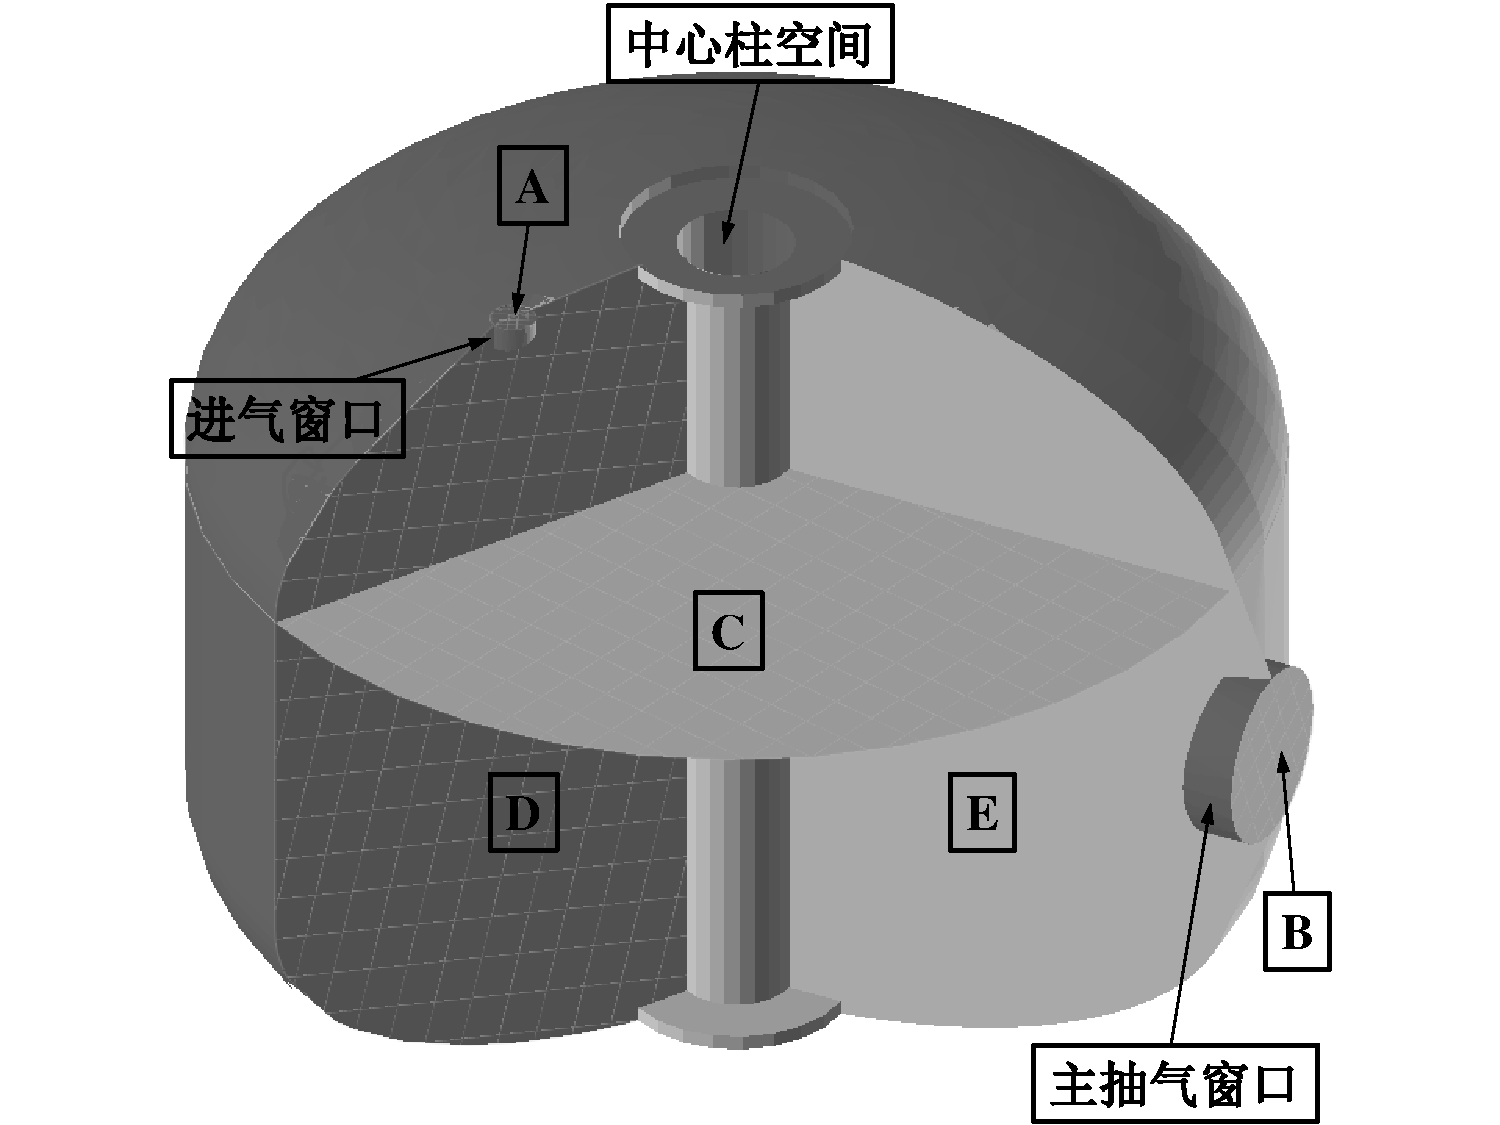
\includegraphics[width=0.6\textwidth]{moflow-vessel.pdf}
  \caption{Molflow+ 模拟使用的 SUNIST 真空室三维模型。共计算了五个截面的气压分布:A)主抽气口截面;B)充气口截面;C)位于赤道面以上,与赤道面平行的环向真空室截面;D)通过充气口中心的极向真空室截面;E)通过主抽气口中心的极向真空室截面。}
  \label{fig:chap04:vv-3d-model}
\end{figure}

A 平面的脉冲出气速率和时常设为 $50\,{\rm Pa}\cdot{\rm L}/{\rm s}$ 和 $100\,{\rm ms}$,B 平面的抽气速率设为 $1200\,{\rm Pa}\cdot{\rm L}/{\rm s}$。模拟中通过对穿过感兴趣截面或在感兴趣截面处反射的粒子数进行统计,完成该截面上的气压分布计算。在放电持续时间很长的托卡马克中,来自壁循环的气体对维持真空室内的粒子数起到重要作用,但是在对 SUNIST 的模拟中,基于以下几点考虑:a)SUNIST的放电时间很短,b)真空室壁材料使用不锈钢并做了很好的抛光处理,c)实验前都会对真空室进行烘烤和辉光放电清洗,d)分子泵的抽速远大于真空室壁的充气速率,e)在长时间连续放电时,壁吸附和解析过程达到平衡,真空室壁设为无壁吸附和解析的漫反射面。

\begin{figure}%[H]
    \centering
    \begin{subfigure}{0.465\columnwidth}
        \begin{overpic}[width=\columnwidth]{fig_6_a.pdf}
          \put(33,1.5){\mbox{\colorbox{white}{\quad 时间}}}
        \end{overpic}
        \caption{}%
        \label{fig:simulation:4}
    \end{subfigure}
    \begin{subfigure}{0.45\columnwidth}
        \fbox{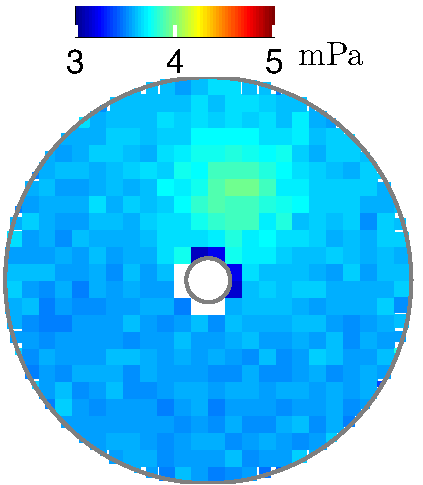
\includegraphics[width=\columnwidth]{fig_6_b.pdf}}
        \caption{}%
        \label{fig:simulation:1}
    \end{subfigure}
    \begin{subfigure}{0.45\columnwidth}
        \fbox{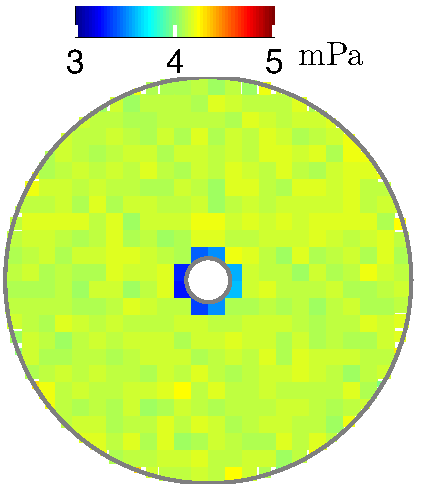
\includegraphics[width=\columnwidth]{fig_6_c.pdf}}
        \caption{}%
        \label{fig:simulation:2}
    \end{subfigure}
    \hspace{1em}
    \begin{subfigure}{0.45\columnwidth}
        \fbox{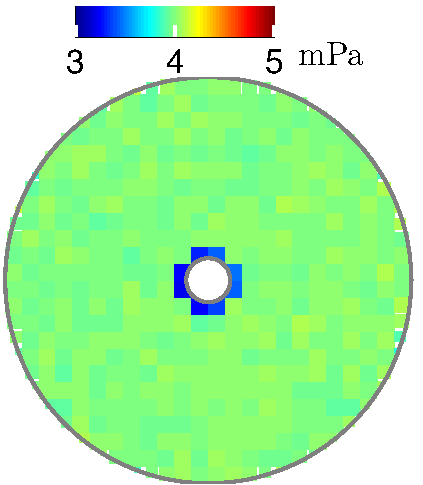
\includegraphics[width=\columnwidth]{fig_6_d.pdf}}
        \caption{}%
        \label{fig:simulation:3}
    \end{subfigure}
    \caption{主抽气口处(图 \ref{fig:chap04:vv-3d-model} 中 C 截面)平均气压和近赤道截面(图 \ref{fig:chap04:vv-3d-model} 中 E 截面)气压分布的 Molflow+ 模拟结果。
    图\ref{fig:simulation:1}、\ref{fig:simulation:2} 和 \ref{fig:simulation:3} 分别对应
    图 \ref{fig:simulation:4} 中的(1)、(2) 和 (3) 时刻。具有与模拟相同进气量的气压实际测量曲线也在图 \ref{fig:simulation:4} 中画出。}%
    \label{fig:simulation}
\end{figure}

主抽气口处(图 \ref{fig:chap04:vv-3d-model} 中 B 截面)平均气压和近赤道截面(图 \ref{fig:chap04:vv-3d-model} 中 C 截面)气压分布的模拟结果在图 \ref{fig:simulation} 中画出。在气压上升阶段,模拟计算的出气口处气压值与实际测量曲线相符(图 \ref{fig:simulation:4})。当进气结束时,模拟气压值呈指数下降趋势,但是气压测量值中存在一个准稳态的平顶区。这是因为在实际装置上,压电阀与进气窗口之间 $300\,{\rm mm}$ 长的充气管道起到了缓冲作用,在进气停止后,管道内的较高压强气体仍然向真空室内充气。

进气脉冲过程中,气压处于快速上升阶段,此时气压在大环方向具有明显的分布不均(图
\ref{fig:simulation:1})。但是,由于气体分子的自由程大于真空室尺度,气体分子会在瞬间到达真空室的各个地方。中心柱也会在一定程度上对气压分布产生影响。当进气脉冲结束时,气压值达到最高,大环方向大尺度的气压不均匀性消失(图 \ref{fig:simulation:2}),但仍然存在小尺度上的气压分布不均匀性。一段时间后,真空室内的气压分布变得均匀(图 \ref{fig:simulation:3})。

真空室内气压流动模拟结果显示,气压分布的演化与气压信号可以紧密联系起来。通过对气压变化过程的测量和分析即可以推测气压分布随时间的变化过程。

\subsection{调整进气时序对 SUNIST 放电重复性的改善}

通过气压信号,对真空室内气体的时间和空间分布演化进行了研究。通过分析,给出了新的进气时序安排。在新的进气时序下,等离子体放电的重复性得到了改善。

\begin{figure}%[H]
  \centering
  \begin{overpic}[width=0.6\textwidth]{mag_field_to_pgas_diff_reacqdata.pdf}
    \put(41,1.5){\mbox{\colorbox{white}{\quad 时间}}}
  \end{overpic}
  \caption{气压信号 $p_{\rm gas}$ 在多种情况下的测量结果。(a)无磁场时的气压信号 $p_{\rm gas}^{{\rm no}B}$ 与正常等离子体放电时的气压信号 $p_{\rm gas}^{I_{\rm p}}$;(b)无磁场时气压信号与只投入一个磁场时的气压信号之差:$\Delta p_{\rm gas}^{B_{\rm t}}=p_{\rm gas}^{B_{\rm t}}-p_{\rm gas}^{{\rm no}B}$,$\Delta p_{\rm gas}^{B_{\rm o}}=p_{\rm gas}^{B_{\rm o}}-p_{\rm gas}^{{\rm no}B}$,$\Delta p_{\rm gas}^{B_{\rm v}}=p_{\rm gas}^{B_{\rm v}}-p_{\rm gas}^{{\rm no}B}$。}
  \label{fig:chap04:mag-to-pgas-diff}
\end{figure}

1)气压信号分析

电离规管暴露在托卡马克的复杂磁场中,一般规管测量所得的气压信号 $p_{\rm gas}$ 在一定程度上会受到影响。所以有必要对气压信号测量进行有效验证。图 \ref{fig:chap04:mag-to-pgas-diff}(b) 画出了在相同的进气脉冲时,只触发欧姆场 $B_{\rm o}$、 环向场 $B_{\rm t}$ 和垂直场 $B_{\rm v}$ 中的一个磁场与无磁场下气压测量信号的差别随时间的变化图。可以看出,$B_{\rm t}$ 与 $B_{\rm v}$ 对气压信号的影响很小,可以忽略。当 $B_{\rm o}$ 投入后,我们发现加入 $B_{\rm o}$ 的 $p_{\rm gas}^{B_{\rm o}}$ 信号相对有 $0.2\times10^{-3}\,{\rm Pa}$ 的下降。主要原因是,当欧姆场投入时,有一小部分气体被电离,气压信号就会相应减小。

在正常等离子体放电中,等离子体电流形成后,真空室内的气体分子被电离并约束在磁场中。分子泵持续抽空无约束等离子体区域。此时的条件即等同于真空室的总体积被大大缩减。所以,气压信号在等离子体形成时开始急速下降(图 \ref{fig:chap04:mag-to-pgas-diff}(a))。等离子体电流形成至气压信号 $p_{\rm gas}^{I_{\rm p}}$ 开始下降约需 $22\,{\rm ms}$。两种机制造成了此延时:首先是气体分子从主真空室流经抽气管道至电离规位置所需的时间;其次是双 T 陷波器对气压信号叠加的相移造成的延时。所以在后续的分析中,要随时计入气压信号相对于主真空室内气压约 $22\,{\rm ms}$ 的延时。

真空室内气压演化可以分为四个阶段(图 \ref{fig:chap04:mag-to-pgas-diff}(a)):第一阶段伴随着脉冲进气过程,称为充气阶段(the puffing stage),此时的气压信号快速上升。第二阶段(缓冲阶段\pozhehao the buffering stage)中,当进气脉冲结束后,气压信号 $p_{\rm gas}$ 需时 $70\,{\rm ms}$ 达到最大值。计入 $p_{\rm gas}$ 本身的 $22\,{\rm ms}$ 延时,缓冲阶段的持续时间为 $48\,{\rm ms}$。正如第 \ref{subsec:vv-related-parts} 节中提到的,缓冲阶段的形成是由在真空室与压电阀之间 $300\,{\rm mm}$ 长的充气管道的缓冲作用形成的。紧跟气压信号最大值的,是一个持续时间约为 $61\,{\rm ms}$ 的准稳态气压平顶(quasi-stationary flat top)阶段。平顶阶段后,气压进入下降阶段(the falling stage),根据文献 \onlinecite{Seo2008:kstar-puffing} 中方程 (1),在下降阶段中气压信号以指数形式下降。

\begin{figure}%[H]
  \centering
  \begin{overpic}[width=0.6\textwidth]{gas_puff_timing_reacqdata_130528.pdf}
    \put(40,1){\mbox{\colorbox{white}{\small \quad 时间}}}
  \end{overpic}
  \caption{调整进气时序前后的 $p_{\rm gas}$ 信号,包括有等离子体放电时 $p_{\rm gas}^{I_{\rm p}}$ 与无等离子体放电时 $p_{\rm gas}^{{\rm no}I_{\rm p}}$ 的气压信号。气压信号的四个阶段也一并在图中画出。}
  \label{fig:chap04:gas-puff-timing}
\end{figure}

2)调整进气时序对 SUNIST 放电重复性的改善

SUNIST 等离子体操作中,常规进气脉冲(gas normal)被安排在欧姆场投入时间前 $5 {\rm ms}$ 结束。然而 $p_{\rm gas}$ 信号显示,在这种进气时序安排下,当等离子体形成时真空室内的气压仍然处于快速上升过程(缓冲阶段),此时仍需 $43\,{\rm ms}$ 的时间 $p_{\rm gas}$ 信号才能达到最大值。我们可以将进气脉冲时序提前 $80\,{\rm ms}$ (gas ahead),在提前进气时序下,在等离子体形成时,气压已经达到平顶段约 $37\,{\rm ms}$ 的时间。此时真空室内的气压分布也已达平衡状态。调整进气脉冲时序前后的 $p_{\rm gas}$ 信号在图 \ref{fig:chap04:gas-puff-timing} 中画出。

使用等离子体物理参数 $P$ 的标准差做为等离子体放电重复性的度量,$t$ 时刻该物理参数的标准差为:
\begin{equation}
  s_{P}(t)=\sqrt{\frac{1}{n-1}\sum_{i=1}^{n}\left(P_i(t)-\overline{P}(t)\right)^2}
  \label{eq:chap04:standard-deviation-of-parameter}
\end{equation}
其中,$n$ 为总放电次数,这里 $P$ 代表等离子体电流 $I_{\rm p}$、电子密度 $n_{\rm e}$ 或单杂环信号 $V_{\rm FL}$ 中的某一参数,$\overline{P}(t)=\sum_i\left(P_i(t)\right)/n$ 为 $t$ 时刻物理量 $P$ 的平均值。

常规进气时序与提前进气时序的离子体电流标准差在图 \ref{fig:chap04:ip-vloop-ne-repeation}(c) 中画出。等离子体放电过程可以分为爬升段(ramping up phase)、平顶段(flat top phase)和下降段(falling phase)三个阶段。将进气提前 $80\,{\rm ms}$ 可以明显改善等离子体电流爬升段和平顶段的可重复性。在 $I_p$ 爬升阶段,$s_{I_p}$ 数据出现了两个峰值,说明爬升段开始与结束时等离子体的重复性较差。将放电过程放在气压的准稳态平顶段后,电流上升段的整体重复性得到了提高,而且第二个 $s_{I_p}$ 峰值消失。当等离子体电流开始下降时,两种进气时序下的 $s_{I_p}$ 曲线趋向相同,意味着改变进气时序并不能改善电流下降段的等离子体重复性。这可能是因为此时欧姆场的加热能力开始剧烈下降引起的。



\subsection{讨论}

SUNIST 托卡马克的充气特性\pozhehao 如充气量与真空室内气压分布等\pozhehao 对放电的可重复性有明显影响。经过细致设计充气系统并对进气时序安排进行调整可以明显改善放电的可重复性,为基于重复放电进行测量的实验提供基本条件。

经分析,以下是影响放电重复性的两个主要因素:

首先,放电时气压分布的均匀性对获得重复放电有重要作用。真空室内气体流动模拟结果显示,在常规进气时序放电中,等离子体放电处于真空室内不均匀分布气压的动态变化阶段。炮与炮之间,这种动态变化的不均匀气压分布状态很难控制到相同的条件,这样每炮之间的等离子体则会产生不一致性。

其次,放电开始时不同的气压值也会对放电重复性造成影响。环向电场与气压的比值 $E/p_{gas}$ 对等离子体放电击穿和电流爬升起到重要作用\cite{Antonio2001:TCABR:breakdown,Chattopa1996:SINP:breakdown}。常规与提前进气时序下,放电开始时的气压值分别为 $4\times10^{-3}\,{\rm Pa}$ 和 $5.5\times10^{-3}\,{\rm Pa}$。SUNIST 放电时,所有的磁场均使用相同的控制条件。那么在相同的环向电场条件下,不同的气压值会影响等离子体击穿和电流爬升过程。

\begin{figure}%[H]
  \centering
  \begin{overpic}[width=0.7\textwidth]{ip_vloop_ne_repeation_reacqdata.pdf}
    \put(30,1.5){\mbox{\colorbox{white}{\quad 时间}}}
  \end{overpic}
  \caption{连续 20 炮放电时的等离子体电流信号:(a)常规进气时序(gas normal)放电;(b)提前 $80\,{\rm ms}$ 进气时序(gas ahead)放电。不同进气时序下的(c)等离子体电流 $I_{\rm p}$、(d)静电探针测量的边界电子密度 $n_{\rm e}$ 与(e)单杂环信号 $V_{\rm FL}$ 的标准差。}
  \label{fig:chap04:ip-vloop-ne-repeation}
\end{figure}

静电探针测量的电子密度 $n_{\rm e}$ 与单杂环信号 $V_{\rm FL}$ 的标准差分别在图 \ref{fig:chap04:ip-vloop-ne-repeation}(d) 和 图 \ref{fig:chap04:ip-vloop-ne-repeation}(e) 中画出。调整进气时序以前的放电中,快速变化的气压为电离过程带来不确定性,进而为等离子体的电子密度带来不确定性。同时气压分布的不均也带来电子密度分布的不均。当等离子体在旋转时,会为在固定位置测量的 $n_{\rm e}$ 信号带来涨落。当调整时序后,等离子体的重复性得到改善,$n_{\rm e}$ 的涨落幅度也降低。在放电平顶段,$n_{\rm e}$ 的标准差从 $\sim1.0\times10^{12}{\rm cm}^{-3}$ 下降至 $\sim0.2\times10^{12}{\rm cm}^{-3}$,且其涨落幅度也消失。对于常规进气时序放电,较差的 $n_{\rm e}$ 重复性导致了等离子体电阻(环电压)的较差重复性。如图 \ref{fig:chap04:ip-vloop-ne-repeation}(e) 所示,调整进气时序可以将单杂环信号 $V_{\rm FL}$ 的相对标准差从 $\sim3.5\%$ 减至 $\sim1.5\%$。

虽然定量分析这些气压因素对放电参数的影响是一个复杂且艰难的工作,但我们可以尽量减小其带来的影响,从而提高实验中放电的可重复性,完成相应的研究工作。
